% !TEX program = lualatex
\documentclass{cfg}

\title{\textsc{Gridworld}}
\author{Jarod DURET\\ Jonathan HENO}
\date{\today}

\begin{document}
\maketitle

\section{Architecture}

\begin{figure}[H]
    \centering
    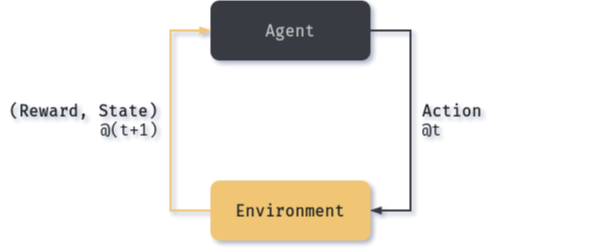
\includegraphics[height=5cm]{img/architecture}
    \caption{Interactions between the decision maker and the environment}
\end{figure}

\section{$\epsilon$-greedy policy}
There is a chance (valued at $\epsilon \in [0;1]$) that an action initially chosen by the agent will not take effect. In our code we call it the \textbf{disobey factor}.
\begin{equation}
    p_{\pi}(s,a) \overset{\Delta}{=} \begin{cases}
        1-\epsilon \quad &\mbox{if $a \in \pi(s)$}\\
        \epsilon / (Card(A) - 1) \quad &\mbox{otherwise}\\
    \end{cases}
\end{equation}
It helps weighting the decision process given the fact that an action can fail and lead to another random decision, and thus to an unplanned reward.
It also helps the agent to widen its field of view, to explore a wider space.

\newpage
\section{Markov Decision Process}
The rewards progressively propagate accross the world and the optimal policy is questioned at each time step, by gauging every possible actions for each state.\\

\begin{algorithmic} 
    \REQUIRE $S(\left\{i|i=0..N^2\right\}),~ A(\{N, E, S, W\}),~ T(S, A) \in S,~ p_{\pi},~ \gamma,~ \epsilon,~ \delta$
    \ENSURE $\mathbf{\pi^\star}(S), \mathbf{v_{\pi}^{\star}}(S)$
    \STATE


    \STATE\COMMENT Initialization
    \STATE $\mathbf{\pi^{\star}_0}(S) \gets (rand(A))_{s \in S}$
    \STATE $\mathbf{v^{\star}_{\mathbf{\pi^{\star}}, 0}}(S) \gets \mathbf{0}$
    \STATE

    \FOR{$t=1$ \TO $t_{obs}$}
        \STATE\COMMENT Policy evaluation
        \STATE $
            \mathbf{v_{\mathbf{\pi^{\star}}, t}}(S) 
            \gets 
            \left(
                \sum\limits_{s^\prime \in T(s, A(s))} 
                p_{\mathbf{\pi^{\star}_{t-1}}}(s, a)\left( 
                    r(s^\prime) 
                    + \gamma v_{\mathbf{\pi^{\star}}, t-1}^{\star}(s^\prime) 
                \right)
            \right)_{a\in\mathbf{\pi^{\star}_{t-1}}(S)}
        $
        \STATE

        \STATE\COMMENT Policy improvement
        \STATE\COMMENT We value all actions available for each state $s \in S$
        \STATE $
            \mathbf{\pi^\star_{t}}(S) 
            \gets 
            \left(
                \underset{a \in A}{argmax}~
                \mathbf{v_{a, t}}(s)
            \right)_{s\in S}
        $
        \STATE $
            \mathbf{v_{\mathbf{\pi^{\star}}, t}^{\star}}(S) 
            \gets 
            \left(
                \underset{a \in A}{max}~
                \mathbf{v_{a, t}}(s)
            \right)_{s \in S}
        $

        \IF{$\max\limits_{s \in S}
            \left(
                \mathbf{v^{\star}_{\mathbf{\pi^{\star}}, t}}(s) - \mathbf{v^{\star}_{\mathbf{\pi^{\star}}, t-1}}(s)
            \right) \leq \delta
        $}
            \RETURN $\mathbf{\pi^\star_t}(S), \mathbf{v_{\mathbf{\pi^{\star}}, t}^{\star}}(S)$
        \ENDIF
    \ENDFOR

    \RETURN $\mathbf{\pi^\star_{t_{obs}}}(S), \mathbf{v_{\mathbf{\pi^{\star}}, t_{obs}}^{\star}}(S)$
\end{algorithmic}
\ 

The other methods rely more on the policy than the previous one.
At each time step, for a given epoch, each action taken, with respect to current policy, is weighted and learned throught environment feedbacks.

\newpage
\section{State Action Reward State Action (SARSA)}
\noindent The key formulae of this algorithm is the following equation:
\begin{equation}
    Q_{s_t, a_t} = Q_{s_t, a_t} + \alpha (R_{s_t, a_t} + \gamma Q_{s_{t+1}, a_{t+1}} - Q_{s_t, a_t})
\end{equation}

With this in mind, in every iteration, we should generate two actions, with respect to the ongoing policy, and get the arrival state of both actions.
We then update the $Q$ matrix with the reward associated with the first action taken in the process: the optimal state is built upon the action value function, by mapping the optimal action given a fixed state.
\begin{algorithmic} 
    \REQUIRE $S(\left\{i|i=0..N^2\right\}),~s_0\in S, ~ A(\{N, E, S, W\}),~ T(S, A) \in S,~ p_{\pi},~ \gamma,~ \epsilon,~ \alpha,~ n_{u, max}$
    \ENSURE $\mathbf{\pi^\star}(S), Q(S)$
    \STATE


    \STATE\COMMENT Initialization
    \STATE $Q^{(0)}, \mathbf{\pi^{\star}_0}(S) \gets (0)_{a\in A, s\in S}, (rand(A))_{s \in S}$
    \STATE $s_0, n_{unchanged} \gets s_0, 0$
    \STATE

    \FOR{$t=0$ \TO $(t_{obs} - 1)$}
        \STATE\COMMENT Generating first action with respect to policy $\mathbf{\pi^{\star}_{t}}$ at state $s_t$
        \STATE $a_t, s^\prime \gets \mbox{\texttt{gen\_move(}} s_{t}, \mathbf{\pi^{\star}_{t}} \mbox{\texttt{)}}$

        \STATE\COMMENT Generating second action with respect to ongoing policy $\mathbf{\pi^{\star}_t}$ from state $s_{t+1}$
        \STATE $a_{t+1}, s^{\prime\prime} \gets \mbox{\texttt{gen\_move(}}s^\prime, \mathbf{\pi^{\star}_t}\mbox{\texttt{)}}$
        \STATE

        \STATE\COMMENT Correcting model given the actions taken
        \STATE $
            Q^{(t+1)}_{s_t, a_t} 
            \gets 
            Q^{(t)}_{s_t, a_t} 
            + \alpha (
                R_{s_t, a_t} + \gamma Q^{(t)}_{s^\prime, a_{t+1}} - Q^{(t)}_{s_t, a_t}
            )
        $

        \STATE\COMMENT Improving policy given the update of the $Q$-values for state $s_t$
        \STATE $
            \mathbf{\pi^{\star}_{t+1}}(s_t) 
            \gets
            \underset{a \in A(s_t)}{argmax}~
            \mathbf{Q_{s_t, a}}(s)
        $
        \STATE

        \STATE\COMMENT Updating next state for next iteration
        \STATE $s_{t+1} \gets s^\prime$
        \STATE

        \IF{$\mathbf{\pi^{\star}_{t+1}} = \mathbf{\pi^{\star}_{t}}$}
            \STATE $n_{unchanged} \gets n_{unchanged} + 1$
            \IF{$n_{unchanged} = n_{u, max}$}
                \RETURN $\mathbf{\pi^\star_{t+1}}(S), Q^{(t+1)}$
            \ENDIF
        \ELSE
            \STATE $n_{unchanged} \gets 0$
        \ENDIF
    \ENDFOR
    \RETURN $\mathbf{\pi^\star_{t_{obs}}}(S), Q^{(t_{obs})}$
\end{algorithmic}
\ 

\noindent And voilà!

\newpage
\section{Q-learning}
\noindent The logic is more or less the same than the previous, except the fact that we are valuing the best action value function in the landing state to optimize the model:
\begin{equation}
    Q_{s_t, a_t} = Q_{s_t, a_t} + \alpha \left(
        R_{s_t, a_t} + \gamma \left(
            \underset{a \in A(s_{t+1})}{max} Q_{s_{t+1}, a} 
        \right) - Q_{s_t, a_t}
    \right)
\end{equation}


\begin{algorithmic} 
    \REQUIRE $S(\left\{i|i=0..N^2\right\}),~s_0\in S, ~ A(\{N, E, S, W\}),~ T(S, A) \in S,~ p_{\pi},~ \gamma,~ \epsilon,~ \alpha,~ n_{u, max}$
    \ENSURE $\mathbf{\pi^\star}(S), Q(S)$
    \STATE


    \STATE\COMMENT Initialization
    \STATE $Q^{(0)}, \mathbf{\pi^{\star}_0}(S) \gets (0)_{a\in A, s\in S}, (rand(A))_{s \in S}$
    \STATE $s_0, n_{unchanged} \gets s_0, 0$
    \STATE

    \FOR{$t=0$ \TO $(t_{obs} - 1)$}
        \STATE\COMMENT Generating first action with respect to policy $\mathbf{\pi^{\star}_{t}}$ at state $s_t$
        \STATE $a_t, s^\prime \gets \mbox{\texttt{gen\_move(}} s_{t}, \mathbf{\pi^{\star}_{t}} \mbox{\texttt{)}}$
        \STATE

        \STATE\COMMENT Correcting model given the actions taken
        \STATE $
            Q^{(t+1)}_{s_t, a_t} 
            \gets 
            Q^{(t)}_{s_t, a_t} 
            + \alpha \left(
                R_{s_t, a_t} 
                + \gamma \left(
                    \underset{a \in A(s^\prime)}{max} Q^{(t)}_{s^\prime, a} 
                \right) 
                - Q^{(t)}_{s_t, a_t}
            \right)
        $

        \STATE\COMMENT Improving policy given the update of the $Q$-values for state $s_t$
        \STATE $
            \mathbf{\pi^{\star}_{t+1}}(s_t) 
            \gets
            \underset{a \in A(s_t)}{argmax}~
            \mathbf{Q_{s_t, a}}(s)
        $
        \STATE

        \STATE\COMMENT Updating next state for next iteration
        \STATE $s_{t+1} \gets s^\prime$
        \STATE

        \IF{$\mathbf{\pi^{\star}_{t+1}} = \mathbf{\pi^{\star}_{t}}$}
            \STATE $n_{unchanged} \gets n_{unchanged} + 1$
            \IF{$n_{unchanged} = n_{u, max}$}
                \RETURN $\mathbf{\pi^\star_{t+1}}(S), Q^{(t+1)}$
            \ENDIF
        \ELSE
            \STATE $n_{unchanged} \gets 0$
        \ENDIF
    \ENDFOR
    \RETURN $\mathbf{\pi^\star_{t_{obs}}}(S), Q^{(t_{obs})}$
\end{algorithmic}
\end{document}